\documentclass{article}
% =======PACKAGES=======
% FORMATTING
\usepackage{amssymb}
\usepackage{amsmath}
\usepackage{breqn}
\usepackage{graphics}
\usepackage{graphicx}
\usepackage{latexsym}
\usepackage{setspace}
\usepackage{hyperref}

\hypersetup{
    colorlinks=true,
    linkcolor=blue,
    filecolor=magenta,      
    urlcolor=cyan,
    pdftitle={Traveling Salesman Problem Approaches},
    pdfpagemode=FullScreen,
}

%\usepackage{algorithm2e}

\usepackage[margin=0.625in]{geometry}
\usepackage{parskip, setspace}
\setstretch{1.15}
\renewcommand{\arraystretch}{1.25}
% TYPESETTING - MATH
\usepackage{amsmath, amsfonts}
\usepackage[ruled, linesnumbered, noend]{algorithm2e}
\RestyleAlgo{ruled}
% RICH
\usepackage{caption}

% BIBLIOGRAPHY
\usepackage{natbib}
\bibliographystyle{unsrt}

% =======TITLE=======
\title{\vspace*{-0.625in}CS 565: Scientific Computing \\ Project 1: Random Search \& Empirical Gradient Descent\vspace*{-0.25in}}
\author{Nathan Chapman, Hunter Lawrence, Andrew Struthers}
\date{\today}

\begin{document}

\maketitle
\tableofcontents
\pagebreak
\textbf{\textit{Honor code: We pledge that we have neither given nor received help from anyone other than the instructor or the TAs for all work components included here. -- Nathan, Hunter, Andrew}}

\section{Introduction}
The Traveling Salesman Problem (TSP) is one of the most extensively studied combinatorial optimization problems in computer science and logistics and operations research. The problem is a standard benchmark for evaluating the efficacy of various combinatorial algorithms. The TSP is seemingly simple in problem statement yet the complexity required in finding the optimal solution is what makes it such a studied problem. The TSP requires finding the shortest possible tour that visits each city in a network of cities exactly once while returning to the starting city. This problem and its many variants are applicable in logistics, transportation planning, and network design, among others.
\\\\
In this paper, we will discuss algorithmic solutions to the TSP, focusing on four prominent heuristic based approaches: Tabu Search, Branch-and-Bound, Simulated Annealing, and Ant Colony Optimization (ACO). Each of these approaches offers a distinct mechanism for navigating the vast solution spaces possible in traveling salesman problems. These algorithms are all inspired by nature, mathematical heuristics, and metaheuristic paradigms.
\begin{itemize}
    \item \textbf{Tabu Search:} 
    \begin{itemize}
        \item Tabu Search is a metaheuristic algorithm introduced by Fred Glover in 1986. This algorithm explores the solution space of a combinatorial optimization problem through iterative improvements while preventing cycling by maintaining a memory structure known as the Tabu list. This list keeps track of recently explored solutions, so that future searches can avoid revisiting these locations. This helps guide the search towards unexplored regions, solving many issues found in other local or neighborhood search algorithms. Tabu Search excels in efficiently navigating complex landscapes, offering a balance between exploration and exploitation.
    \end{itemize}

    \item \textbf{Branch-and-Bound:}
    \begin{itemize}
        \item Branch-and-Bound originated in operations research and it provides a systematic technique for solving optimization problems by recursively partitioning the solution space into smaller subspaces. Using bounding, pruning, and branching processes, Branch-and-Bound can remove unpromising regions of the search space, significantly reducing the computational burden. Branch-and-Bound guarantees optimality, as all promising areas of the search space are explored, but this comes at the expensive cost of increased computational complexity. As such, this algorithm is only practical for smaller problem instances.
    \end{itemize}

    \item \textbf{Simulated Annealing:}
    \begin{itemize}
        \item This algorithm is inspired by the annealing process in metallurgy. Simulated Annealing is a probabilistic metaheuristic algorithm that is capable of mimicking the gradual cooling of molten metal with the goal of resting at a low-energy crystalline state. To do this, the algorithm will traverse the solution space by allowing occasional uphill moves to escape local optima, where the acceptable worse solutions are bounded by a temperature parameter. The temperature parameter will gradually decrease over time, which allows escape from local optima early on in pursuit of a better final resting point. Simulated Annealing is capable of escaping local optima, which many simpler algorithms struggle with. However, just like most other algorithms, Simulated Annealing does not guarantee global optimality.
    \end{itemize}

    \item \textbf{Ant Colony Optimization (ACO):}   
    \begin{itemize}
        \item ACO is one of the many particle swarm algorithms, and it is modeled after the foraging behavior of ants. This algorithm is a population-based metaheuristic algorithm that uses swarm intelligence to guide the search process. Ants deposit pheromones along their paths, which will influence the choices of subsequent ants based on the concentration of pheromones. This iterative process converges towards optimal or near-optimal solutions. Using pheromone evaporation will help to ensure that the ants actually explore the space, and don't just exploit one good path found early on in the iteration process.
    \end{itemize}
\end{itemize}

\begin{figure}[h]
    \centering
    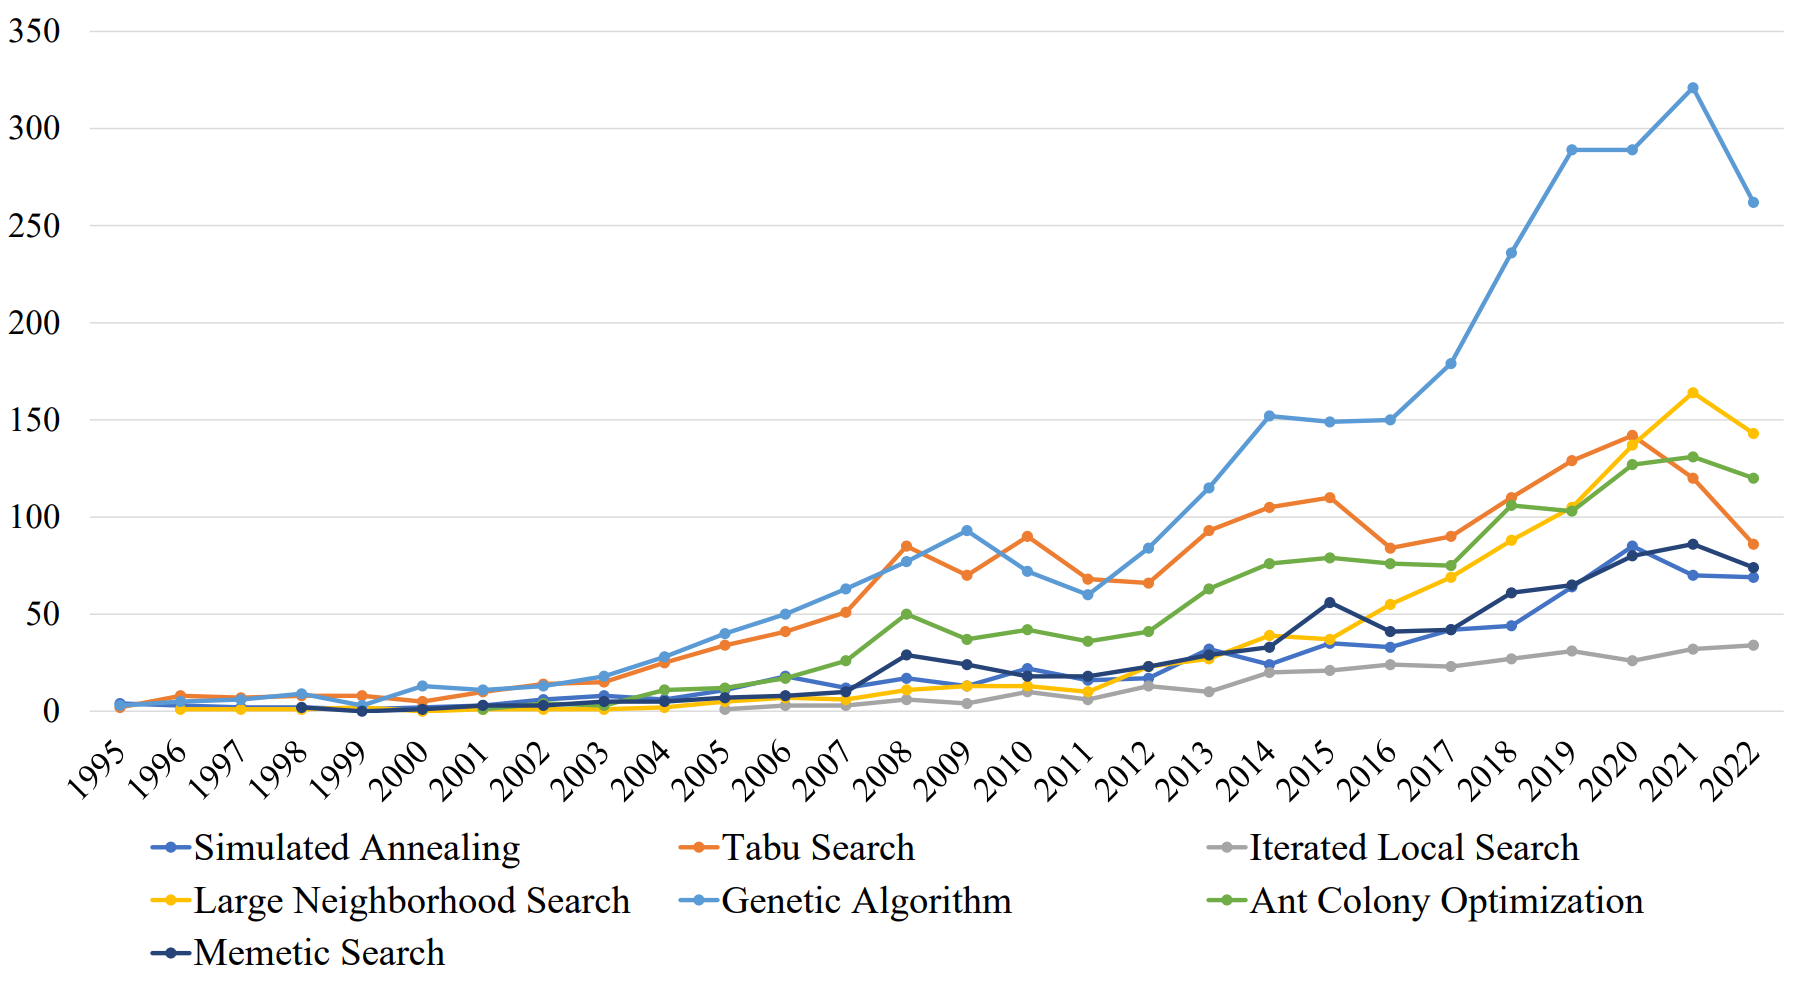
\includegraphics[width=\textwidth,keepaspectratio]{Images/TSPAlgs.PNG}
    \caption{Publications using different heuristic algorithms to solve TSP/VRP instances}
    \label{fig:algsOverTime}
\end{figure}

\noindent We can see in the figure above that interest and number of publications using some of these algorithms has grown substantially in the last decade. Up until 2019-2020, Tabu Search, for example, was one of the most popular approaches to the TSP. Ant Colony Optimization has also received more and more attention as computational power continues to increase. 


\section{Algorithms}


\subsection{Tabu Search}
Tabu Search is a powerful metaheuristic algorithm that can efficiently explore solution spaces while avoiding stagnation in local optima. Tabu Search introduces the concept of a ``tabu list" which guides the search process. The Tabu list prevents the algorithm from revisiting previously explored solutions, which helps the algorithm avoid getting stuck in local minima while also reducing computational complexity. The Tabu list can be set up to ``forget" solutions after a certain duration, or if some condition is met, so that the algorithm can continue making effective progress. This memory-based mechanism enables Tabu Search to reach a really good balance between exploration and exploitation while preventing getting stuck in local minima. This makes Tabu search much more effective at finding high quality solutions compared to other greedy, local, or neighborhood based searches.

\subsubsection{Key Concepts}
Some of the key components of this algorithm are the neighborhood exploration, the Tabu list management, and aspiration criteria. Tabu Search begins with an initial solution and explores neighboring solutions within some neighborhood. The Tabu list then stores information about recent solutions, preventing the algorithm from revisiting them in subsequent iterations. Entries in the Tabu list can expire after a certain number of iterations if we desire. This can help promote exploration by not preventing solutions from never being revisited once new information is learned. Each iteration of the algorithm requires Tabu Search to evaluate the objective function, so that it can assess the quality of candidate solutions. In certain cases, Tabu Search may override the Tabu status of a move if it leads to a superior solution. This aspiration mechanism allows the algorithm to consider otherwise forbidden moves under favorable conditions, further promoting exploration and an ability to escape from local optima.
\begin{figure}[h]
    \centering
    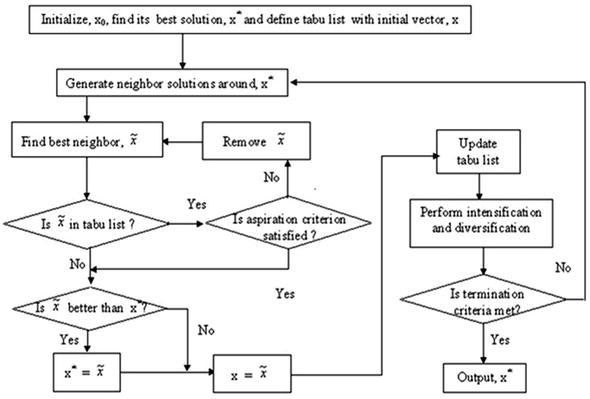
\includegraphics[width=0.55\textwidth,keepaspectratio]{Images/tabu.png}
    \caption{A visual flowchart for the Tabu Search algorithm}
    \label{fig:algsOverTime}
\end{figure}

\noindent Tabu Search provides a good balance between exploration and exploitation, allowing an adaptive approach to solving combinatorial optimization problems such as the TSP. By incorporating memory-based mechanisms and efficient neighborhood exploration, Tabu Search can efficiently navigate solution spaces and escaping local optima to solve the TSP effectively. 


\subsubsection{Algorithm}
This algorithm works by iteratively improving upon some initial solution by exploring neighboring solutions within a defined neighborhood structure. The algorithm maintains a Tabu list, which records recently visited solutions. By incorporating memory into the search process, Tabu Search can escape local optima and explore diverse regions of the solution space without repeating previously searched areas. A pseudocode implementation of the algorithm is shown below:

\begin{algorithm}[!h]
    \DontPrintSemicolon
    \caption{Tabu Search}
    \label{alg:tabu}
    \KwResult{An optimized solution to the TSP using Tabu search}

    $current\_solution \gets \{\}$\;
    $tabu\_list \gets \{\}$\;
    \While{Stopping criteria is not met}
    {
        $candidate\_solutions \gets$ set of candidate solutions within the neighborhood of $current\_solution$\;
        $best\_solution\gets\{\}$\;
        \ForEach{$solution \in candidate\_solutions$}
        {
            \If{$solution$ is better than $best\_solution$ and $solution \notin tabu\_list$}
            {
                $current\_solution \gets solution$\;
            }
        }
        Add $current\_solution$ to $tabu\_list$\;
        Perform Tabu list management strategies such as aging and aspiration\;
    }
    \Return{$current\_solution$}
\end{algorithm}
\newpage


\subsection{Branch-and-Bound}
Branch-and-Bound is a classic algorithmic technique that systematically partitions the solution space into smaller, manageable subspaces. Branch-and-Bound uses a divide-and-conquer strategy coupled with bounding techniques to prune unpromising regions of the search space, ultimately converging towards an optimal solution.


\subsubsection{Key Concepts}
Branch-and-Bound offers a systematic and rigorous approach to solving the TSP by partitioning the solution space into manageable subspaces and pruning unpromising regions. Despite its computational overhead, Branch-and-Bound guarantees optimality or near-optimality for the TSP, making it an incredibly powerful tool. The main drawback is that the systematic analysis of many possible routes as the problem size increases can drastically impact runtime efficiency, where large instances can run for hundreds of CPU years, and thousands of real-time hours.
\begin{figure}[h]
    \centering
    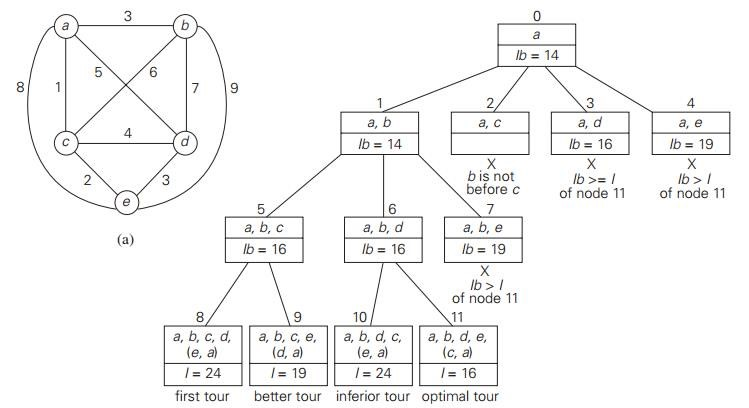
\includegraphics[width=0.55\textwidth,keepaspectratio]{Images/bnb.jpg}
    \caption{The Branch-and-Bound algorithm creating branches of tours starting at node $a$}
    \label{fig:bandb}
\end{figure}

\noindent The core strategies with this algorithm are the ability to branch, bound, and prune the solution trees. At each iteration, Branch-and-Bound selects a branching variable or decision to partition the solution space into smaller subspaces. Then, Branch-and-Bound uses bounding techniques to establish upper and lower bounds on the objective function within each subspace. These bounds allow the algorithm to prune entire branches of the search tree if they cannot possibly lead to an optimal solution, thus reducing the computational complexity. Branch-and-Bound traverses the search tree in a depth-first manner, systematically exploring branches until a termination criterion is met. The algorithm employs backtracking to backtrack from dead-end branches and continue exploration in other parts of the tree. This results a guaranteed global optima being found. We traverse until either no valid branches are left, or we have checked the whole tree. Either way, the global optima will be found. This operation is costly, however, as the size of the problem grows.

\subsubsection{Algorithm}
The Branch-and-Bound algorithm operates by recursively subdividing the search space into subspaces and bounding the feasible region of each subspace based on certain criteria. With the bounding of subspaces, the algorithm iteratively searches until the optimal solution is identified or all subspaces have been exhausted. The bounds are calculated by objective function value of each branch, which can allow the efficient pruning of subspaces that cannot possibly contain an optimal solution.

\begin{algorithm}[!h]
    \DontPrintSemicolon
    \caption{Branch-and-Bound}
    \label{alg:bnb}
    \KwResult{Solution to the TSP disregarding subspaces that can't yield an optimal outcome.}

    $best\_solution\gets\{\}$\;
    $best\_cost\gets \infty$\;
    $priority\_queue\gets\{starting\_vertex\}$\;
    \While{$priority\_queue$ is not empty}
    {
        $node \gets$ element of $priority\_queue$ with lowest cost\;
        \If{$node$ is a leaf}
        {
            \If{$node$ cost $<best\_cost$}
            {
                Update $best\_solution$ and $best\_cost$\;
            }
        }
        \Else
        {
            \ForEach{$child\_node\in node$}
            {
                \If{$child\_node$ is feasible}
                {
                    $lower\_bound \gets $ lower bound of objective function for child node\;
                    $upper\_bound\gets$ upper bound of objective function\;
                    \If{$lower\_bound \leq best\_cost$}
                    {
                        Add $child\_node$ to $priority\_queue$\;
                    }
                }
            }
        }
    }
    \Return{$best\_solution$}\;
\end{algorithm}
\newpage



\subsection{Simulated Annealing}
Simulated Annealing is a probabilistic metaheuristic algorithm inspired by the annealing process in metallurgy, where a material is gradually cooled to reach a low-energy state. Simulated Annealing was introduced by Kirkpatrick et al. in 1983 and mimics the stochastic behavior of atoms in a cooling system. By allowing occasional uphill moves, controlled by a temperature parameter, Simulated Annealing can navigate uphill in the solution space to escape local optima and converge towards optimal or near-optimal solutions.

\subsubsection{Key Concepts}
The Simulated Annealing algorithm relies on a temperature schedule, neighborhood exploration, acceptance criteria, and a cooling schedule. The algorithm must track a temperature parameter that controls the probability of accepting worse solutions. The temperature decreases over time according to a predefined cooling schedule, typically exponential or logarithmic, simulating the annealing process. Higher temperatures facilitate exploration by allowing uphill moves, while lower temperatures encourage exploitation by favoring downhill moves. At each iteration, Simulated Annealing generates neighboring solutions by applying local modifications to the current solution. Common neighborhood structures include 2-opt, 3-opt, or k-opt moves in the context of the TSP. Simulated Annealing probabilistically accepts or rejects candidate solutions based on their quality and the current temperature. Moves that improve the objective function are always accepted, while worse moves are accepted with a probability determined by some criterion, which relates the change in objective function value to the current temperature. Finally, the cooling schedule dictates the rate at which the temperature decreases over iterations. A slower cooling schedule allows for more exploration in the early stages of the search, while a faster cooling schedule intensifies exploitation towards the later stages. The choice of cooling schedule impacts the algorithm's convergence behavior and solution quality.

\subsubsection{Algorithm}
Simulated Annealing operates iteratively, simulating the annealing process through a sequence of temperature-dependent transformations. At each iteration, the algorithm explores neighboring solutions and probabilistically accepts or rejects moves based on their impact on the objective function and the current temperature. As the temperature decreases over time, the likelihood of accepting worse solutions diminishes, leading to convergence towards a global optimum.

\begin{algorithm}[!h]
    \DontPrintSemicolon
    \caption{Simulated Annealing}
    \label{alg:anneal}
    \KwData{$initial\_solution$ is the seed solution, $initial\_temperature$ is the starting temperature of the solution, $cooling\_schedule$ is the rate of temperature decrease}
    \KwResult{}

    $current\_solution\gets initial\_solution$\;
    $temperature \gets initial\_temperature$\;
    \While{$temperature > 0$}
    {
        $new\_solution \gets$ some neighbor of $current\_solution$\;
        $delta\_cost \gets$ $objective(new\_solution) - objective(current\_solution)$\;
        \If{$delta\_cost < 0$ or $rand < e^{\frac{-delta\_cost}{temperature}}$}
        {
            $current\_solution\gets new\_solution$\;
        }
        $temperature\gets cooling(temperature)$\;
    }
    \Return{$current\_solution$}
\end{algorithm}

\begin{figure}[h]
    \centering
    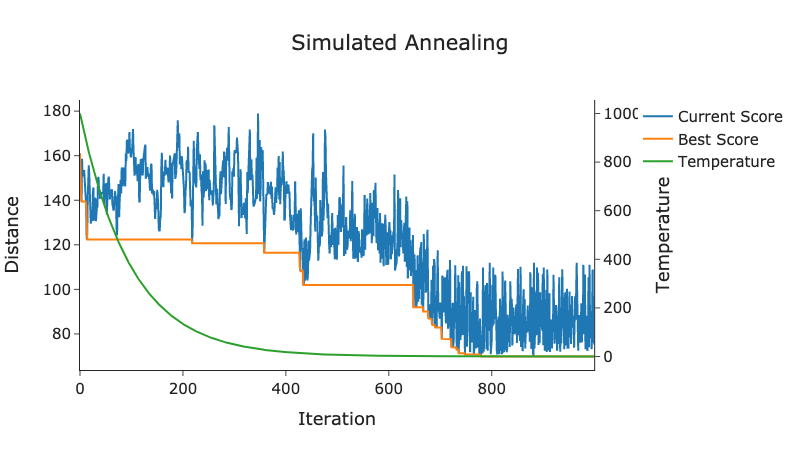
\includegraphics[width=1\textwidth,keepaspectratio]{Images/SA.png}
    \caption{Sample of the Simulated Annealing algorithm improving a solution to the TSP over 1000 iterations}
    \label{fig:bandb}
\end{figure}

\noindent Simulated Annealing offers a powerful and versatile approach to optimization by emulating the annealing process in metallurgy. In the figure above we can see an example implementation of Simulated Annealing where the temperature of the system decreases exponentially. The current score increases and decreases wildly in the first few hundred iterations, but as the temperature decreases the solution starts to converge on an optimal solution. The best score started at \~160, and after \~700 iterations it had decreased by about 50. Once the temperature fell enough, the algorithm was able to improve the solution by roughly the same delta of 50 while only taking around 75 iterations. This shows how the gradual cooling of the system allows the system to explore many solutions initially and converge as the iterations increase.

\subsection{Ant Colony Optimization}
Ant Colony Optimization offers a powerful and adaptive approach to solving combinatorial optimization problems by harnessing the collective intelligence of swarms. ACO is a population-based metaheuristic algorithm inspired by the foraging behavior of ants. ACO is a particle swarm algorithm that leverages the principles of swarm intelligence to solve the TSP very effectively. By simulating the foraging behavior of ants, ACO constructs solutions by probabilistic decision-making and pheromone communication. Each ant follows a pheromone trail that influences its decisions each time it reaches a vertex in the TSP graph.

\subsubsection{Key Concepts}
The foundation of ACO is built with pheromone trails, ant behavior, local search and construction, and pheromone updates including evaporation over time. Pheromone trails represent the collective memory of the ant colony and guide the exploration of the solution space. Initially, pheromone trails are uniformly distributed. As ants traverse paths, they deposit pheromones, with the quantity proportional to the quality of the solution found. Pheromone evaporation ensures adaptability and prevents premature convergence. Ants probabilistically select paths based on a combination of pheromone information and heuristic knowledge. The pheromone trail intensifies the attractiveness of paths with higher pheromone concentrations, while heuristic information guides exploration towards promising regions of the solution space. Ants may employ stochastic decision rules such as probabilistic selection of paths using some random generation to encourage exploration and not just blindly following the ants that came before. Ants construct solutions incrementally by selecting and appending components of partial solutions. We can then use some simple local search mechanisms, such as 2-opt or 3-opt, to try and improve on the found solution, but this step isn't necessary. After each iteration, pheromone trails are updated to reflect the quality of constructed solutions. Pheromone evaporation will ensure the decay of pheromone concentrations over time, preventing stagnation and promoting exploration. Additionally, pheromone reinforcement is applied to paths traversed by high-quality solutions, intensifying their attractiveness to subsequent ants.

\begin{figure}[h]
    \centering
    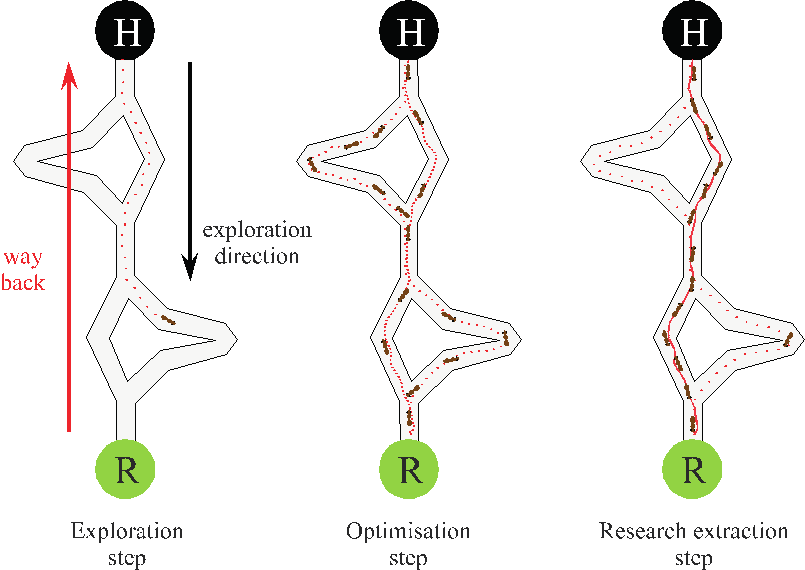
\includegraphics[width=0.75\textwidth,keepaspectratio]{Images/aco.jpg}
    \caption{Ants finding the optimal path from the start to the finish in a simple graph}
    \label{fig:ant}
\end{figure}

\subsubsection{Algorithm}
ACO operates by iteratively constructing candidate solutions using a population of virtual ants. Each ant probabilistically selects paths based on the pheromone trails deposited by previous ants. As ants traverse paths, they deposit pheromones, which influence the decisions of subsequent ants. Over time, the concentration of pheromones on promising paths increases, guiding the exploration towards better solutions.
\begin{algorithm}[!h]
    \DontPrintSemicolon
    \caption{Ant Colony Optimization}
    \label{alg:aco}
    \KwResult{}

    Initialize $pheromone\_trails$\;
    Initialize parameters\;
    $best\_solution\gets\{\}$\;
    \While{Stopping criteria is not met}
    {
        \tcc{Construct solutions for each ant}
        \ForEach{$ant\in all\_ants$}
        {
            Initialize ant memory\;
            $visited\_set\gets\{\}$\;
            Randomly select a $start\_node$\;
            Add $start\_node$ to $visited\_set$\;

            \While{$||visited\_set|| < all\_nodes$}
            {
                Probabilistically select next component in solution based on pheromone trails and heuristic information\;
                Update $visited\_set$\;
                Update pheromone trails\;
            }
        
            Apply local search to ant memory\;
            \If{solution is better than $best\_solution$}
            {
                $best\_solution\gets$ solution\;
            }
        
            Update pheromone trails based on solution quality\;
        }
        Evaporate pheromone trails\;
    }
    
    \Return{$best\_solution$}
\end{algorithm}

\newpage
\section{Comparison}
Each algorithm we have discussed possesses distinct characteristics that influence its performance in terms of solution quality, convergence, and computational efficiency.
\\\\
Tabu Search is great at efficiently navigating solution spaces while preventing stagnation in local optima through the use of memory-based mechanisms. It often produces high-quality solutions, converging relatively quickly with effective Tabu list management. While computationally efficient for moderate-sized problems, Tabu Search may struggle to find the global optimum for highly complex or multimodal problems.
\\\\
In contrast, Branch-and-Bound guarantees optimal solutions for the TSP, ensuring the highest possible solution quality. It exhibits strong convergence properties, particularly in the TSP and its variants. However, its computational overhead is quite large, and in larger problem instances this can severely limit efficiency and solution generation within a feasible time window.
\\\\
Simulated Annealing explores solution spaces probabilistically, escaping local optima through controlled exploration. It converges towards optimal or near-optimal solutions, especially with appropriately tuned cooling schedules. Simulated Annealing's computational efficiency and scalability make it suitable for large and complex problems, but solution quality may vary depending on parameter settings and problem characteristics. The cooling rate, number of iterations, and tolerance for bad solutions greatly impacts Simulated Annealing's ability to find the global optima. Even so, it is very commonly used in industry applications as it is generally very reliably good. 
\\\\
Ant Colony Optimization harnesses the collective intelligence of an ant colony to construct solutions iteratively. It often produces high-quality solutions by effectively exploring diverse regions of the solution space through pheromone communication. ACO exhibits strong convergence properties and, as a particle swarm algorithm, is highly parallelizable and scalable. This makes ACO suitable for large problems where Tabu search and Branch-and-Bound start to struggle. However, this algorithm has many parameters that require careful tweaking in order to generate high quality solutions that converge quickly.

\section{Conclusion}
In conclusion, each algorithm offers unique strengths and weaknesses depending on problem size, computational resources, and desired quality of solution for amount of effort put into tuning the system. The analysis of Tabu Search, Branch-and-Bound, Simulated Annealing, and Ant Colony Optimization allows us to gauge their strengths and weaknesses when generating solutions for the TSP and its many variations. Each algorithm presents a distinct approach to navigating solution spaces, offering trade-offs between solution quality, convergence, and computational efficiency. 
\pagebreak
\nocite*{}
\bibliography{references}


\end{document}
